\documentclass[12pt]{report}
\usepackage[a4paper,left=2.5cm,right=3cm,top=2.5cm,bottom=2.5cm]{geometry}
\usepackage{titlesec}
\usepackage{amssymb}
\usepackage{amsmath}
\usepackage{amsthm}
\usepackage{amsfonts}
\usepackage{thmtools}
\usepackage{cleveref}
\usepackage[shortlabels]{enumitem}
\usepackage{array}
\usepackage{pgffor}
\usepackage{xcolor}
\usepackage{tikz}
\usetikzlibrary{automata,positioning}
\tikzstyle{accepting}=[double distance=2pt,outer sep=1pt+\pgflinewidth]
\tikzset{>=latex}

\newcommand{\sectionbreak}{\clearpage}
\setlist[enumerate,1]{label={(\alph*)}}

% let the theorem title have the same attribute as the theorem heading
\makeatletter
\def\th@definition{
  \thm@notefont{}
  \normalfont
}
\makeatother

% different types of "theorems"
\declaretheorem[style=definition,numberwithin=chapter]{theorem}
\declaretheorem[style=definition,sibling=theorem]{proposition}
\declaretheorem[style=definition,sibling=theorem]{lemma}
\declaretheorem[style=definition,sibling=theorem]{corollary}
\declaretheorem[style=definition,sibling=theorem]{definition}
\declaretheorem[style=definition,numbered=no]{example}
\declaretheorem[style=definition,numbered=no]{examples}
\declaretheorem[style=definition,numbered=no]{notation}
\declaretheorem[style=definition,numbered=no]{remark}

% use bold fonts to emphasize
\DeclareTextFontCommand{\emph}{\boldmath\bfseries}

\begin{document}
\chapter{Regular Languages}
\section{Strings and Languages}
\begin{definition}
  An \emph{alphabet} is a finite set of symbols.
  A \emph{string} over alphabet $\Sigma$ is a finite sequence
  \begin{equation*}
    w = a_1 a_2 \cdots a_n
  \end{equation*}
  with $a_1, \dots, a_n \in \Sigma$, where $n$ is called the \emph{length} of
  the string $w$.
  The \emph{empty string} is the unique string of length zero, which is denoted
  by $\epsilon$.
\end{definition}

\begin{definition}
  The \emph{concatenation} of strings
  \begin{equation*}
    u = a_1 a_2 \cdots a_n
    \quad \text{and} \quad
    v = b_1 b_2 \cdots b_m
  \end{equation*}
  is defined as the string
  \begin{equation*}
    uv = a_1 a_2 \cdots a_n b_1 b_2 \cdots b_m.
  \end{equation*}
\end{definition}

\begin{definition}
  Let $\Sigma^*$ denote the set of all strings over $\Sigma$.
  A subset of $\Sigma^*$ is called a \emph{language} over $\Sigma$.
\end{definition}

\begin{definition}
  The \emph{concatenation} of languages $L_1$ and $L_2$ is
  \begin{equation*}
    L_1L_2 = \{w_1w_2 : \text{$w_1 \in L_1$ and $w_2 \in L_2$}\}.
  \end{equation*}
  For any language $L$, we define $L^0 = \{\epsilon\}$ and $L^{n+1} = L^nL$
  for all integers $n \geq 0$.
  Also, we define $L^* = \bigcup_{n \geq 0}L^n$.
\end{definition}

\section{Deterministic Finite State Automata}
\begin{definition}
  A \emph{deterministic finite state automaton (DFA)} is a 5-tuple
  \begin{equation*}
    M = (Q, \Sigma, \delta, s, F),
  \end{equation*}
  where each component is as follows.
  \begin{itemize}
    \item $Q$ is a finite set of \emph{states}.
    \item $\Sigma$ is an alphabet.
    \item $\delta: Q \times \Sigma \to Q$ is a \emph{transition function}.
    \item $s \in Q$ is the \emph{start state}.
    \item $F \subseteq Q$ is the set of \emph{final states}.
  \end{itemize}
\end{definition}

%\begin{definition}
%  Let $A = (Q, \Sigma, \delta, q_0, F)$ be a DFA.
%  For each string $w \in \Sigma^*$, we define $\delta_w: Q \to Q$ as follows,
%  where $a \in \Sigma$ and $x \in \Sigma^*$.
%  \begin{itemize}
%    \item $\delta_\epsilon(p) = p$ for each $p \in Q$.
%    \item $\delta_a(p) = \delta(p, a)$ for each $p \in Q$.
%    \item $\delta_{xa}(p) = \delta(\delta_x(p), a)$ for each $p \in Q$.
%  \end{itemize}
%\end{definition}

\begin{definition}
  Let $A = (Q, \Sigma, \delta, q_0, F)$ be a DFA.
  \begin{itemize}
    \item We say that $A$ accepts a string $w \in \Sigma^*$ if
    $\delta_w(q_0) \in F$.
    \item The \emph{language} of $A$, denoted $L(A)$, is defined as the set of
    strings that are accepted by $A$.
  \end{itemize}
\end{definition}

\begin{definition}
  A language $L$ is \emph{regular} if there exists a DFA $A$ such that
  $L(A) = L$.
\end{definition}

\begin{example}
  Let $A = (\{q_0, q_1\}, \{0, 1\}, \delta, q_0, \{q_1\})$ be a DFA, where the
  transition function $\delta$ is as follows.
  \begin{center}
    \begin{tabular}{c|cc}
      & 0 & 1 \\
      \hline
      $q_0$ & $q_0$ & $q_1$ \\
      $q_1$ & $q_0$ & $q_1$
    \end{tabular}
  \end{center}
  Instead of using the formal definition, one can also draw a state diagram of
  $A$ as follows.
  \begin{center}
    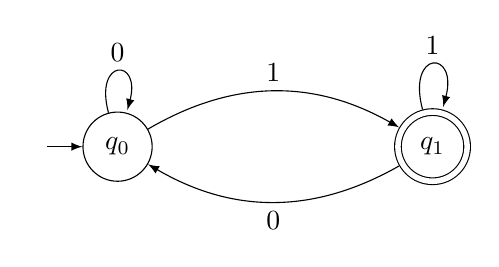
\begin{tikzpicture}[every state/.style={initial text=}]
      \node[state,initial] (q0) at (0, 0) {$q_0$};
      \node[state,accepting] (q1) at (4, 0) {$q_1$};
      \path[->] (q0) edge[loop above] node[above] {0} (q0);
      \path[->] (q0) edge[bend left] node[above] {1} (q1);
      \path[->] (q1) edge[loop above] node[above] {1} (q0);
      \path[->] (q1) edge[bend left] node[below] {0} (q0);
    \end{tikzpicture}
  \end{center}
  It can be shown that a string $w \in \{0, 1\}^*$ is accepted by $A$ if and
  only if $w$ ends with $1$.
  Thus, the language $L = \{w \in \{0, 1\}^* : \text{$w$ ends with 1} \}$
  is regular.
\end{example}

\begin{theorem}
  If $L$ is a regular language over $\Sigma$, then $\Sigma^* \setminus L$
  is also regular.
\end{theorem}
\begin{proof}
  Let $A = (Q, \Sigma, \delta, q_0, F)$ be a DFA with $L = L(A)$.
  Let $A' = (Q, \Sigma, \delta, q_0, Q \setminus F)$.
  Then for each $w \in \Sigma^*$, we have
  \begin{equation*}
    w \in L(A')
    \quad \Leftrightarrow \quad \delta_w(q_0) \in Q \setminus F
    \quad \Leftrightarrow \quad w \notin L(A).
  \end{equation*}
  Thus, $L(A') = \Sigma^* \setminus L(A)$, implying that $\Sigma^* \setminus L$
  is regular.
\end{proof}

\begin{theorem}
  \label{thm:regular-union}
  If $L_1$ and $L_2$ are regular languages over $\Sigma$, then $L_1 \cup L_2$
  is also regular.
\end{theorem}
\begin{proof}
  Let
  \begin{equation*}
    A_1 = (Q_1, \Sigma, \delta^{(1)}, q_1, F_1)
    \quad \text{and} \quad
    A_2 = (Q_2, \Sigma, \delta^{(2)}, q_2, F_2)
  \end{equation*}
  be DFAs with $L_1 = L(A_1)$ and $L_2 = L(A_2)$.
  We construct the DFA
  \begin{equation*}
    A = (Q_1 \times Q_2, \Sigma, \delta, (q_1, q_2), F)
  \end{equation*}
  as follows.
  \begin{itemize}
    \item $\delta((p, q), a) = (\delta^{(1)}(p, a), \delta^{(2)}(q, a))$ for
    each $p \in Q_1$, $q \in Q_2$ and $a \in \Sigma$.
    \item $F = \{(p, q): \text{$p \in F_1$ or $q \in F_2$}\}$.
  \end{itemize}
  It can be shown that for each string $w \in \Sigma^*$, we have
  \begin{align*}
    w \in L(A)
    &\quad \Leftrightarrow \quad \delta_w((q_1, q_2)) \in F \\
    &\quad \Leftrightarrow \quad \text{$\delta^{(1)}_w(q_1) \in F_1$ or
    $\delta^{(2)}_w(q_2) \in F_2$} \\
    &\quad \Leftrightarrow \quad \text{$w \in L(A_1)$ or $w \in L(A_2)$}.
  \end{align*}
  Thus, $L(A) = L(A_1) \cup L(A_2)$, implying that $L_1 \cup L_2$ is regular.
\end{proof}

\begin{corollary}
  If $L_1$ and $L_2$ are regular languages over $\Sigma$, then $L_1 \cap L_2$
  is also regular.
\end{corollary}
\begin{proof}
  Straightforward since by De Morgan's law we have
  \begin{equation*}
    L_1 \cap L_2
    = \Sigma^* \setminus
    ((\Sigma^* \setminus L_1) \cup (\Sigma^* \setminus L_2)).
    \qedhere
  \end{equation*}
\end{proof}

\section{Nondeterministic Finite State Automata}
\begin{definition}
  \label{def:nfa}
  A \emph{nondeterministic finite state automaton} (NFA) is a tuple
  \begin{equation*}
    A = (Q, \Sigma, \delta, q_0, F),
  \end{equation*}
  where each component is as follows.
  \begin{itemize}
    \item $Q$ is a finite set of \emph{states}.
    \item $\Sigma$ is a finite set of input symbols.
    \item $\delta \subseteq Q \times \Sigma \times Q$ is a relation, called the
    \emph{transition relation}.
    \item $q_0 \in Q$ is called the \emph{start state}.
    \item $F \subseteq Q$ is called the \emph{accepting states}.
  \end{itemize}
\end{definition}

\begin{definition}
  Let $A = (Q, \Sigma, \delta, q_0, F)$ be an NFA.
  For each string $w \in \Sigma^*$, we define $\delta_w \subseteq Q \times Q$
  as follows, where $a \in \Sigma$ and $x \in \Sigma^*$.
  \begin{itemize}
    \item $\delta_\epsilon = \{(p, q): p = q\}$.
    \item $\delta_a = \{(p, q): (p, a, q) \in \delta\}$.
    \item $\delta_{xa} = \{(p, q): \text{$(p, r) \in \delta_x$ and
    $(r, q) \in \delta_a$ for some $r \in Q$}\}$.
  \end{itemize}
\end{definition}

\begin{definition}
  Let $A = (Q, \Sigma, \delta, q_0, F)$ be an NFA.
  \begin{itemize}
    \item We say that $A$ accepts a string $w \in \Sigma^*$ if there exists
    $q \in F$ such that $(q_0, q) \in \delta_w$.
    \item The \emph{language} of $A$, denoted $L(A)$, is defined as the set of
    strings that are accepted by $A$.
  \end{itemize}
\end{definition}

\begin{theorem}
  For every NFA $A$, there is a DFA $A'$ with $L(A') = L(A)$.
\end{theorem}
\begin{proof}
  Let $A = (Q, \Sigma, \delta, q_0, F)$.
  We construct $A' = (\mathcal{P}(Q), \Sigma, \Delta, \{q_0\}, \Phi)$
  as follows.
  \begin{itemize}
    \item $\Delta: \mathcal{P}(Q) \times \Sigma \to \mathcal{P}(Q)$ is the
    function with
    \begin{equation*}
      \Delta_a(P) = \bigcup_{p \in P} \; \{q \in Q: (p, q) \in \delta_a\}
    \end{equation*}
    for any $P \subseteq Q$ and $a \in \Sigma$.
    \item $\Phi = \{P \subseteq Q: P \cap F \neq \varnothing\}$.
  \end{itemize}
  Now we prove that for any $w \in \Sigma^*$, for any $q \in Q$ and for any
  $P \subseteq Q$, we have $q \in \Delta_w(P)$ if and only if
  $(p, q) \in \delta_w$ for some $p \in P$.
  For the induction basis, let $w = \epsilon$, and we have
  \begin{equation*}
    q \in \Delta_\epsilon(P)
    \quad \Leftrightarrow \quad
    q \in P
    \quad \Leftrightarrow \quad
    \text{$(p, q) \in \delta_\epsilon$ for some $p \in P$}.
  \end{equation*}

  For the induction step, let $w = xa$, where $x$ is any string and $a$ is any
  symbol.
  Note that by the construction of $\Delta$, we have $q \in \Delta_a(P)$ if and
  only if $(p, q) \in \delta_a$ for some $p \in P$.
  Thus, we can conclude that
  \begin{align*}
    q \in \Delta_{xa}(P)
    \quad &\Leftrightarrow \quad
    q \in \Delta_a(\Delta_x(P)) \\[.5em]
    \quad &\Leftrightarrow \quad
    \text{$(r, q) \in \delta_a$ for some $r \in \Delta_x(P)$} \\
    &\hspace*{2.6em} \text{and $(p, r) \in \delta_x$ for some $p \in P$}
    \\[.5em]
    \quad &\Leftrightarrow \quad
    \text{$(p, q) \in \delta_{xa}$ for some $p \in P$}.
  \end{align*}

  Finally we prove that $L(A') = L(A)$, which is given by
  \begin{align*}
    w \in L(A')
    \quad &\Leftrightarrow \quad
    \Delta_w(\{q_0\}) \in \Phi \\[.5em]
    \quad &\Leftrightarrow \quad
    \Delta_w(\{q_0\}) \cap F \neq \varnothing \\[.5em]
    \quad &\Leftrightarrow \quad
    \text{$q \in \Delta_w(\{q_0\})$ for some $q \in F$} \\[.5em]
    \quad &\Leftrightarrow \quad
    \text{$(p, q) \in \delta_w$ for some $q \in F$ and $p \in \{q_0\}$} \\[.5em]
    \quad &\Leftrightarrow \quad
    \text{$(q_0, q) \in \delta_w$ for some $q \in F$} \\[.5em]
    \quad &\Leftrightarrow \quad
    w \in L(A).
    \qedhere
  \end{align*}
\end{proof}

\begin{theorem}
  \label{thm:regular-concatenation}
  If $L_1$ and $L_2$ are regular languages over $\Sigma$, then $L_1L_2$
  is also regular.
\end{theorem}
\begin{proof}
  Let $A_1 = (Q_1, \Sigma, \delta^{(1)}, q_1, F_1)$ and
  $A_2 = (Q_2, \Sigma, \delta^{(2)}, q_2, F_2)$ be NFAs such that
  $L_1 = L(A_1)$ and $L_2 = L(A_2)$.
  We construct an NFA
  \begin{equation*}
    A = (Q_1 \cup Q_2, \Sigma, \delta, q_1, F)
  \end{equation*}
  as follows.
  \begin{itemize}
    \item $\delta = \delta^{(1)} \cup \delta^{(2)} \cup
    \{(p, a, q) \in Q \times \Sigma \times Q:
    \text{$p \in F_1$ and $(q_2, a, q) \in \delta^{(2)}$}\}$.
    \item If $q_2 \in F_2$, let $F = F_1 \cup F_2$. Otherwise, let $F = F_2$.
  \end{itemize}
  It can be shown that $L(A) = L(A_1)L(A_2)$, and thus $L_1L_2$ is regular.
\end{proof}

\begin{theorem}
  \label{thm:regular-closure}
  If $L$ is a regular language over $\Sigma$, then $L^*$ is also regular.
\end{theorem}
\begin{proof}
  Let $A = (Q, \Sigma, \delta, q_0, F)$ be an NFA with $L = L(A)$.
  We construct an NFA
  \begin{equation*}
    A' = (Q \cup \{q_0'\}, \Sigma, \delta', q_0', F \cup \{q_0'\})
  \end{equation*}
  with
  \begin{equation*}
    \delta' = \delta \cup \{(p, a, q) \in Q \times \Sigma \times Q:
    \text{$p \in F \cup \{q_0'\}$ and $(q_0, a, q) \in \delta$}\}.
  \end{equation*}
  It can be shown that $L(A') = (L(A))^*$, and thus $L^*$ is regular.
\end{proof}

\section{Regular Expressions}
\begin{definition}
  Let $\Sigma$ be an alphabet.
  A \emph{regular expression} over $\Sigma$ is a string in the minimal language
  over $\Sigma \cup \{\varnothing, \epsilon, {}^*, +, (, )\}$
  that satisfies the following conditions.
  \begin{enumerate}[1.]
    \item $\varnothing$ is a regular expression.
    \item $\epsilon$ is a regular expression.
    \item If $a \in \Sigma$, then $a$ is a regular expression.
    \item If $e_1$ and $e_2$ are regular expressions, then so is $(e_1e_2)$.
    \item If $e_1$ and $e_2$ are regular expressions, then so is
    $(e_1 + e_2)$.
    \item If $e$ is a regular expression, then so is $(e)^*$.
  \end{enumerate}
\end{definition}

\begin{definition}
  A regular expression $e$ over an alphabet $\Sigma$ defines a language $L(e)$
  as follows.
  \begin{enumerate}[1.]
    \item $L(\varnothing) = \varnothing$.
    \item $L(\epsilon) = \{\epsilon\}$.
    \item $L(a) = \{a\}$ for each $a \in \Sigma$.
    \item $L((e_1e_2)) = L(e_1)L(e_2)$ for each regular expressions $e_1$ and
    $e_2$.
    \item $L((e_1 + e_2)) = L(e_1) \cup L(e_2)$ for each regular
    expressions $e_1$ and $e_2$.
    \item $L((e)^*) = L(e^*)$ for each regular expression $e$.
  \end{enumerate}
\end{definition}

\begin{remark}
  From now on, we may omit parentheses if there is no ambiguity.
\end{remark}

\begin{lemma}
  \label{thm:regex-to-regular}
  If $e$ is a regular expression over an alphabet $\Sigma$, then $L(e)$ is
  regular.
\end{lemma}
\begin{proof}
  It can be easily shown that $\varnothing$ and $\{\epsilon\}$ are regular.
  Moreover, $\{a\}$ is regular for each $a \in \Sigma$.
  Thus, by \Cref{thm:regular-union}, \Cref{thm:regular-concatenation} and
  \Cref{thm:regular-closure}, we can conclude that for all regular expressions
  $e$, $L(e)$ is regular.
\end{proof}

\begin{lemma}
  \label{thm:regular-to-regex}
  If $L$ is a regular language over an alphabet $\Sigma$, then there is a
  regular expression $e$ over $\Sigma$ such that $L(e) = L$.
\end{lemma}
\begin{proof}
  Since $L$ is regular, there exists a DFA $A = (Q, \Sigma, \delta, q_0, F)$
  with $L(A) = L$.
  Suppose that $Q = \{p_1, p_2, \dots, p_n\}$ with $p_1 = q_0$.
  For any $i, j \in \{1, \dots, n\}$ and for any $k \in \{0, \dots, n\}$,
  let $L_{ij}^{(k)}$ denote the language of strings $w$ such that 
  \begin{itemize}
    \item $\delta_w(p_i) = p_j$, and
    \item for each string $x$ with $\epsilon \sqsubset x \sqsubset w$, we have
    $\delta_x(p_i) = p_\ell$ for some $\ell \in \{1, \dots, k\}$.
  \end{itemize}
  We are going to prove that for all $i, j \in \{1, \dots, n\}$ and
  $k \in \{0, \dots, n\}$, there exists a regular expression $e_{ij}^{(k)}$
  such that
  \begin{equation*}
    L\bigl(e_{ij}^{(k)}\bigr) = L_{ij}^{(k)}.
  \end{equation*}

  The proof is by induction on $k$. For the induction basis, let $k = 0$.
  Let $\Pi_{ij} \subseteq \Sigma$ denote the set of symbols $a$ with
  $\delta_a(p_i) = p_j$.
  If $i \neq j$, we have
  \begin{equation*}
    L_{ij}^{(0)} = \bigcup_{a \in \Pi_{ij}} \{a\},
  \end{equation*}
  and thus we can construct $e_{ij}^{(0)}$ by
  \begin{equation*}
    e_{ij}^{(0)} = \sum_{a \in \Pi_{ij}} a.
  \end{equation*}
  (If $\Pi_{ij} = \varnothing$, then the summation is defined as
  $\varnothing$.)
  If $i = j$, we have
  \begin{equation*}
    L_{ii}^{(0)} = \{\epsilon\} \cup \bigcup_{a \in \Pi_{ii}} \{a\},
  \end{equation*}
  and thus we can construct $e_{ii}^{(0)}$ by
  \begin{equation*}
    e_{ii}^{(0)} = \epsilon + \sum_{a \in \Pi_{ii}} a.
  \end{equation*}

  Now for the induction step, let $k \geq 1$.
  Suppose that $w \in L_{ij}^{(k)}$.
  If there is no string $x$ with $\epsilon \sqsubset x \sqsubset w$
  such that $\delta_x(p_i) = p_k$, then we have
  \begin{equation*}
    w \in L_{ij}^{(k-1)}.
  \end{equation*}
  Otherwise, let $x_0, x_1, \dots, x_\ell$ be all strings with
  $\epsilon \sqsubset x_0 \sqsubset x_1 \sqsubset \cdots \sqsubset x_\ell
  \sqsubset w$ such that
  \begin{equation*}
    \delta_{x_0}(p_i)
    = \delta_{x_1}(p_i)
    = \cdots
    = \delta_{x_\ell}(p_i)
    = p_k.
  \end{equation*}
  Let $u_0, u_1, \dots, u_{\ell+1}$ be strings such that
  \begin{equation*}
    w = u_0u_1 \cdots u_{\ell+1},
  \end{equation*}
  and $x_h = u_0u_1 \cdots u_h$ for each $h \in \{0, \dots, \ell\}$.
  Since $u_0 \in L_{ik}^{(k-1)}$, $u_{\ell+1} \in L_{kj}^{(k-1)}$, and
  $u_h \in L_{kk}^{(k-1)}$ for each $h \in \{1, \dots, \ell\}$,
  it follows that
  \begin{equation*}
    w \in L_{ik}^{(k-1)}\left(L_{kk}^{(k-1)}\right)^*L_{kj}^{(k-1)}.
  \end{equation*}
  As a result, we have
  \begin{equation*}
    L_{ij}^{(k)} \subseteq L_{ij}^{(k-1)} \cup
    L_{ik}^{(k-1)}\left(L_{kk}^{(k-1)}\right)^*L_{kj}^{(k-1)},
  \end{equation*}
  implying
  \begin{equation*}
    L_{ij}^{(k)} = L_{ij}^{(k-1)} \cup
    L_{ik}^{(k-1)}\left(L_{kk}^{(k-1)}\right)^*L_{kj}^{(k-1)}.
  \end{equation*}
  Therefore, we can construct $e_{ij}^{(k)}$ by
  \begin{equation*}
    e_{ij}^{(k)} = e_{ij}^{(k-1)}
    + e_{ik}^{(k-1)}\left(e_{kk}^{(k-1)}\right)^*e_{kj}^{(k-1)}.
  \end{equation*}

  Now we can construct the regular expression $e$ with $L(e) = L$ as follows.
  Let $\Phi$ be the set of integers $j \in \{1, \dots, n\}$ such that
  $p_j \in F$.
  Since
  \begin{equation*}
    L = \bigcup_{j \in \Phi} L_{1j}^{(n)},
  \end{equation*}
  we can construct $e$ by
  \begin{equation*}
    e = \sum_{j \in \Phi} e_{1j}^{(n)},
  \end{equation*}
  which completes the proof.
\end{proof}

\begin{theorem}
  Let $\Sigma$ be an alphabet.
  A language $L$ over $\Sigma$ is regular if and only if there is a regular
  expression $e$ over $\Sigma$ such that $L(e) = L$.
\end{theorem}
\begin{proof}
  Straightforward by \Cref{thm:regex-to-regular} and
  \Cref{thm:regular-to-regex}.
\end{proof}
\end{document}